\section{Evaluation}

% \begin{itemize}
%     \item Macro-benchmark
%         \begin{itemize}
%             \item BMC
%                 \begin{itemize}
%                     \item Expressiveness: how to evaluate?
%                         \begin{itemize}
%                             \item LOC: we have 33\% reduction
%                             \item 1 rust program vs 7 eBPF programs
%                             \item based on experience?
%                             \item Rust is a safer language
%                         \end{itemize}
%                     \item Performance evaluation
%                         \begin{itemize}
%                             \item Check their paper to see if we can perform
%                                 the same experiment
%                             \item We want a figure similar to Figure 6 in BMC
%                                 (except we don't need to evaluate on different
%                                 CPU configs)
%                             \item x: Vanilla memcached, BMC, Rust
%                             \item y: normalized throughput
%
%                         \end{itemize}
%                 \end{itemize}
%             \item Electrode
%                 \begin{itemize}
%                     \item LOC reduction
%                     \item Performance using their benchmark (similar to figure
%                         5 and 7 in Electrode)
%                     \item Dynamic allocation (ask the authors)
%                 \end{itemize}
%             \item LSM implementation (if we have time / requires handle
%                 nesting)
%             \item XRP
%             \item FUSE in eBPF (from Hubertus)
%         \end{itemize}
%     \item Micro-benchmark
%         \begin{itemize}
%             \item Memory footprint (BPF vs Rust) given we have a larger binary
%                 \begin{itemize}
%                     \item Number of prog in the same translation unit vs memory
%                         usage for program allocation
%                     \item This is because we are always statically linked to
%                         the runtime crate on the translation unit basis
%                     \item E.g. a bpf kern.c with 4 programs vs a rust main.rs
%                         with 4 programs
%                 \end{itemize}
%             \item Small expressiveness examples
%                 \begin{itemize}
%                     \item Loop: strcmp
%                     \item need more
%                 \end{itemize}
%             \item Stack-check overhead
%                 \begin{itemize}
%                     \item Use BMC?
%                     \item Or create some other workload that are function call
%                         intensive (since our instrumentation happens before
%                         each function call)
%                 \end{itemize}
%             \item Cleanup overhead on normal execution path (recording
%                 allocated kernel objects)
%                 \begin{itemize}
%                     \item Similar to Stack-check
%                 \end{itemize}
%             \item Startup overhead due to stack switching
%                 \begin{itemize}
%                     \item A minimal program () to show the upper bound?
%                     \item Plus a real world application (again BMC)?
%                 \end{itemize}
%         \end{itemize}
% \end{itemize}
\subsection{Usability evaluation}
\subsection{Performance evaluation}
\subsubsection{Memory footprint (BPF vs Rust)}
\begin{figure}
    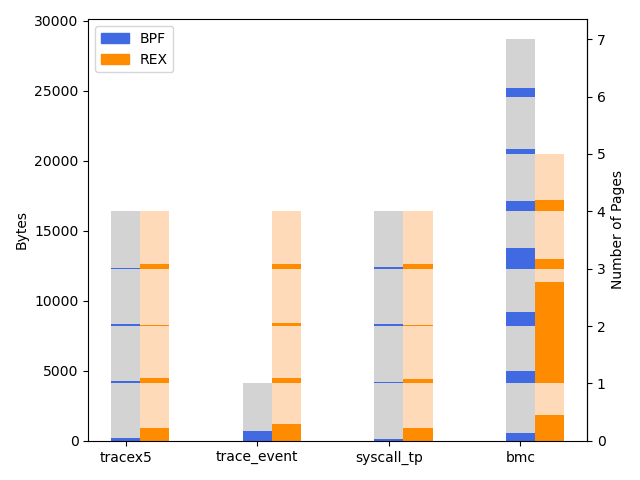
\includegraphics[width=1.0\linewidth]{figs/mem-footprint.png}
    \centering
    \vspace{-25pt}
    \caption{Amount of static memory used by various eBPF and \projname{}
        programs \jinghao{TODO: replot}}
    \label{fig:eval-mem-footprint}
    \vspace{-10pt}
\end{figure}
% definition of memory footprint
% eBPF only have JIT code
% Rust have code sections and other sections, e.g. data and GOT sections
We evaluate on how large the in-kernel memory footprint of \projname{} programs
    is comparing to that of eBPF programs.
We define the memory footprint as the number of static memory pages required
    for program execution.
For eBPF, this only includes the JIT-ed native code, since eBPF program does
    not support static data sections.
% For \projname{} this includes all load segments from the compiled ELF
%     executable, which consists not only the text sections, but also the data
%     sections for static variables (e.g., program objects and maps objects) as
%     well as the sections that implement support for position-independent code
%     (e.g., GOT sections).
For \projname{} this includes all load segments from the compiled ELF
    executable.
A compiled \projname{} program has four load segments, which generally maps to
    relocations, text, read-only data, and the GOT.

In this experiment, we compare the number of memeory pages required for both
    \projname{} programs and their equivalent eBPF programs.
We select 3 simple eBPF programs from the sample eBPF programs shipped with the
    kernel -- the trace point program \texttt{syscall\_tp}, the kprobe program
    \texttt{tracex5} and the perf event program \texttt{trace\_event}.
We also include the BMC program (\S~\ref{eval:macro}) in the experiment because
    it represents an example of a complicated eBPF program.
For all the programs, we implement a \projname{} version with the same
    overall logic.

The memory footprint and the internal breakdowns of various eBPF and
    \projname{} programs are shown in Figure~\ref{fig:eval-mem-footprint}.
In general, the memory footprint becomes more efficient for \projname{} when
    more programs are defined in the same source file. \jinghao{or should we
    say ``project''}
This is because, for eBPF, each program is loaded independently and occupies its
    own pages; \projname{}, on the other hand, allows multiple programs to be
    loaded at once in the same executable, which is in a more condensed form.
\texttt{trace\_event} represents a cases where only a single extension program
    is defined.
For such cases, \projname{} would exhibit a larger memory footprint, because
    its executable contains other sections (e.g., data and relocations) in
    addition to code.
\texttt{tracex5} and \texttt{syscall\_tp} uses the same number of memory pages
    since each of them consists of 4 programs, and one papge per program for
    the eBPF implementation.
For BMC, \projname{} achieves a more efficient memory footprint.
The original eBPF-BMC has to be split into 7 programs in order to keep it
    within the instruction limit of the verifier.
Doing so makes each program occupy its own pages.
The \projname{}-BMC does not need to be split due to the absence of the
    verifier, and therefore utilizes the memory more efficiently.

% \begin{itemize}
%     \item need a figure: bar graph showing the memory footprint of bpf and
%         \projname{} programs on our sample programs
%     \item sample programs: \texttt{syscall\_tp}, \texttt{tracex5},
%         \texttt{trace\_event}, and BMC.
%     \item y: total number of pages allocated for the loaded object (JIT-ed code
%         for BPF, loaded and mapped pages for Rust)
% \end{itemize}

\subsubsection{Startup overhead due to stack switching}
\begin{table}[t]
    \small
    \centering
    \begin{tabular}{ccc}%{|p{6cm}|p{1cm}|}
        \toprule
        \textbf{Extension} & \textbf{Empty prog runtime} & \textbf{Spinlock runtime} \\
        \midrule
        eBPF & 43.5 $\pm$ 4.79 & 256.8 $\pm$ 142.4\\
        \projname{} & 44.1 $\pm$ 4.93 & 254.5 $\pm$ 192.3\\
        \bottomrule
    \end{tabular}
    \caption{Empty program runtime as well as spinlock acquire and release
        runtime for eBPF and \projname{} in nanoseconds}
    \vspace{-10pt}
    \label{tab:startup-overhead}
\end{table}

\projname{}'s usage of a dedicated stack for execution and the implementation
    of exception handling support may incur additional overhead during program
    startup and shutdown.
This design requires saving of the stack and frame pointer and replacing them
    with the top address of the dedicated stack before starting the program,
    and restoring the saved stack and frame pointer after the program exits.
The manipulation of the stack pointers adds to six more memory instructions to
    the dispatcher function of the \projname{} programs.
In this experiment we measure the overhead of these stack pointer operations.
We implement an empty kprobe extension program -- both in eBPF and in
    \projname{} -- and measure their wall runtime including the program
    dispatcher function.
The result is shown in Figure~\ref{tab:startup-overhead}.
On average, the difference of runtime of invoking an empty \projname{} and eBPF
    program is less than 1ns.
This shows the additional stack manipulations needed by \projname{} does not
    contributed to non-negligible overhead.

\subsubsection{Verifier/JIT-based optimization}
\label{eval:inline}

% The raw data and script used to make the graph (plot2.py)
% is in the map-test directory under testing/analysis/
% With the three files: ['elapsed_times_5.15.csv',
%    'elapsed_times_5.15_non_inlined.csv', 'elapsed_times3-rust.csv']
% Corresponding to the bars
% Link to it: https://github.com/rosalab/map-test/tree/main/testing/analysis

\begin{figure}
    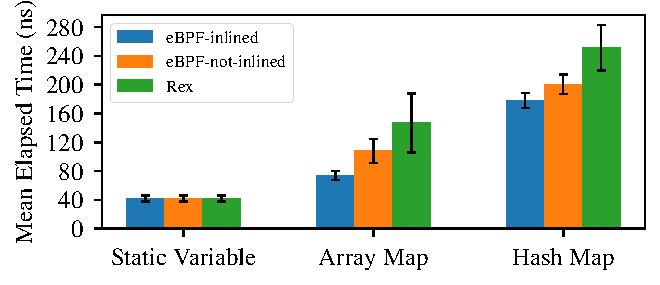
\includegraphics[width=1.0\linewidth]{figs/inline.pdf}
    \centering
    \vspace{-25pt}
    \caption{Runtime of map lookups on various setups}
    \label{fig:eval-inline}
    \vspace{-10pt}
\end{figure}

% \begin{itemize}
%     \item inline v.s. out-of-line map helpers
%         \begin{itemize}
%             \item table showing runtime of a map lookup operation in a eBPF and
%                 a Rust program
%             \item the kernel will automatically inline lookup in BPF
%             \item Rust version will not get inlined
%             \item measurement can be in ns for now, but better if it could be
%                 in cycles
%             \item maps to test: array, hash (htab-lru, xsk-map?)
%         \end{itemize}
% \end{itemize}

We evaluate the impact of missed opportunities due to the elimination of the
    eBPF verifier in \projname{}.
Specifically, we look into the optimization of eBPF map lookups.
For eBPF programs, the verifier can inline the \texttt{bpf\_map\_lookup\_elem}
    helper function by replacing the call into equivalent eBPF instructions.
This optimization can avoid two function calls and two pointer dereferences for
    map types that support lookup inlining.
However, in \projname{}, inlining is not performed due to the absence of the
    eBPF verifier as well as kernel internal information (e.g. map addresses).

In this experiment we measure the runtime of eBPF map lookups under three
    settings, eBPF with inlining, eBPF without inlining, and \projname{}.
Our test program for both eBPF and \projname{} is a tracepoint program that
    uses the \texttt{bpf\_ktime\_get\_ns} helper to measure the runtime of
    a \texttt{bpf\_map\_lookup\_elem} call.
The \texttt{bpf\_map\_lookup\_elem} invocation is by defualt inlined by the
    eBPF verifier when possible.
The setup of eBPF without inlining is achieved by removing the inlining logic
    from the eBPF verifier.
We selected two commonly-used eBPF map types for this experiment: array maps
    and hash maps.
Both of them support lookup inlining.

% Figure~\ref{fig:eval-inline}
% shows the performance of inlining and non-inlining on a vanilla
% v5.15 kernel as well as the \projname{} implementation.
Figure~\ref{fig:eval-inline} shows the performance of map lookups under the
    three different setups on different maps.
% The vanilla non-inlined
% kernel is achieved by commenting out the lines in the kernel verifier.c file that
% automatically inlines the bpf\_map\_lookup\_elem method.
For both array maps and hash maps, the
    runtime of map lookup can be reduced by 20-30 ns compared to eBPF without
    inlining.
% In the graph,
% the performance impact of inlining the method is 20-30 nanoseconds.
% The additional slowdown of 30-40 nanoseconds seen in the rust implementation
% can be explained by the wrapping performed around the bpf\_map\_lookup\_elem method.
An additional slowdown of 30-40 nanoseconds is present for map lookups in
    \projname{}.
This is because of the wrapping code around the kernel
    \texttt{bpf\_map\_lookup\_elem} that allows \projname{} programs to invoke
    it using safe Rust objects.

% Egor: Not sure if I should go into more technical details about whats going on
% in the wrapping

% Using libbpf (and libiu in the case of \projname{}) the sample \projname{} or c bpf
% program is loaded and attached to a tracepoint which is then called by the trigger.
% In the instance of the inlined and non-inlined tests this tracepoint is getcwd, and
% in the instance of the rust tests that tracepoint used is sys\_enter\_dup. The
% triggers consist of a one-line c program that calls the appropriate function such as getcwd().
% The bpf program creates the corresponding map and measures the time
% it takes to execute a single map\_lookup\_elem. This time is measured with
% bpf\_ktime\_get\_ns() and then printed with bpf\_printk() and recorded.
% \milo{Maybe we should talk about why we chose these specific maps. i.e. that array and hash maps are the main ones that support the inlining?}

\subsubsection{Stack-check overhead}
\begin{itemize}
    \item table showing runtime of two programs using small recursion
    \item eBPF: use tail calls for recursion
    \item Rust: just a recursive function
    \item The recursion count should not be statically known to prevent llvm
        from optimizing out the recursion
\end{itemize}

We then evaluate how much overhead the runtime stack check have on the
    performance of \projname{} programs.
The stack instrumentation is added before each
    function call in the \projname{} program if the program contains indirect
    or recursive function calls that prevents the compiler from calculating the
    stack usage statically.
In this experiment we implement recursive factorial computation program in both
    eBPF and \projname{}.
Since eBPF does not natively support recursive functions, we use eBPF tail
    calls to invoke the same program.
At same time, because recursive factorial computation can always be tail-call
    optimized in Rust, this comparison should be able to precisely highlight
    the performance implication of the runtime stack instrumentation.
\jinghao{TODO: discuss results.}

\subsubsection{Cleanup overhead on normal execution path}
% \begin{table}[t]
%     \small
%     \centering
%     \begin{tabular}{cc}%{|p{6cm}|p{1cm}|}
%         \toprule
%         \textbf{Extension} & \textbf{Runtime of acquiring \& release a lock (ns)} \\
%         \midrule
%         eBPF & 256.8 $\pm$ 142.4 \\
%         \projname{} & 254.5 $\pm$ 192.3 \\
%         \bottomrule
%     \end{tabular}
%     \caption{Runtime of spinlock acquire and release for eBPF and \projname{}}
%     \vspace{-10pt}
%     \label{tab:cleanup-overhead}
% \end{table}
The cleanup mechanism employed by \projname{} requires recording the allocated
    resource at runtime, which comparing to eBPF or Itanium C++ ABI, adds extra
    runtime overhead.
We therefore evaluate the runtime overhead from \projname{}'s cleanup
    mechanism.
For this miscrobenchmark, we choose to use a program that acquires and then
    immediately releases a BPF spinlock.
Since the acquired spinlock is a resource that needs to be released upon Rust
    panics, \projname{}'s cleanup mechanism needs to record it in its per-CPU
    buffer.
The program is implemented both in eBPF and \projname{} and the time used to
    acquire and release the spinlocks are measured.
As shown in Table~\ref{tab:cleanup-overhead}, the runtime difference between
    eBPF and \projname{} is less than 2ns with \projname{} being the faster
    one, implying the overhead of \projname{}'s cleanup mechanism is
    negligible.

\subsubsection{\projname{}-BMC}
\label{eval:macro}
We now demonstrate that \projname{} can be used to implement complicated,
    real-world kernel extension use cases with enhanced usability but without
%    losing much performance by implementing BMC and Electrode in \projname{}.
    losing much performance by implementing the BPF Memcached Cache (BMC) in
    \projname{}.

% \subsubsection{\projname{}-based BMC}
% \jinghao{TODO: Preamable}
% BMC implements in-kernel memcached cache -- how it works
% Compilcated program, original paper splits into 7 programs and uses tail calls
%

BMC~\cite{BMC} is an in-kernel cache for Memcached based on eBPF.
It stores recently queried key-value pairs in an eBPF map to accelerate the
    processing of GET requests to the Memcached server.
If a GET is hit in the cache, the queried value can be sent in a reply without
    going through the expensive network stack in the Linux kernel.
The map that servers as the cache is managed by eBPF programs, which implements
    the lookup and update logics.

On the aspect of implementation, BMC is a much more complicated program
    comparing to other common eBPF use cases.
In order to pass the verifier, the implementation has to be splitted into seven
    eBPF programs that tail-calls into each other to reduce verification
    complexity.
Similar problem also presents when processing the incoming packet data, where
    the authors had to bound data size to reduce verification complexity for
    loops.

We re-implement BMC in \projname{} (\projname{}-BMC) to demonstrate the
    enhanced usability without losing performance.
The resulting program is not a direct translation from the original eBPF
    version in C, rather, we implement the same high-level logic but with
    slight deviations from BMC where the enhanced usability and expressiveness
    of Rust allows a simpler implementation.

% The BMC has many places where for loops are nested into different ifs.
% And, due to the limitations of C, many operations do not have built-in functions
%     that can be used directly.

\begin{figure}
    \lstinputlisting[language=myC]{./snippets/s6-bmc.c}
    \caption{Packet parsing code for cache invalidation in BMC}
    \label{fig:bmc-code}
\end{figure}
\begin{figure}
    \lstinputlisting[language=Rust]{./snippets/s6-rust.rs}
    \caption{Packet parsing code for cache invalidation in \projname{}}
    \label{fig:rust-code}
\end{figure}

In the initial design of \projname{}-BMC, the underlying assumption was that
    we should follow the logic of BMC.
But the cache invalidation function Figure~\ref{fig:bmc-code} in BMC employs
    \texttt{for} loops with cumbersome condition checks, and is further
    complicated by the nesting of multiple \texttt{if} statements.
The complexity is exacerbated by introducing two additional variables to track
    the state of key and SET command.
Such complex checks are intentionally designed to pass the
    verifier, but they significantly increase the programming burden
    of BMC, while also leading to readability issues in some places regarding
    the intended functionality.
\jinghao{Add some sentence saying this is a prevalent pattern in BMC?}
% \jinghao{Can we make the claim that this complexity is for passing the
%     verifier?}
% During implementation of function \texttt{bmc\_invalidate\_cache},
%     we assume that each pcket

% This discovery highlighted the obscurity and susceptibility to errors inherent
%     in the original code structure, primarily due to the complex judgment
%     conditions buried within nested if statements.

To address all ``loops'' in BMC, \projname{}-BMC utilizes the lazy-evaluated
    \texttt{windows}, \texttt{enumerate} and \texttt{filter\_map} from slice iterators.
\jinghao{refer back to eBPF code: The same logic is implemented in
    \projname{}-BMC as shown in Figure bla}
These methods in Figure~\ref{fig:rust-code} split the whole payload into chunks
    with 4 bytes, and collects the results for which the chunk equals the keyword
    of SET commands
% \jinghao{What are these challenges -- are we still in the context of cache
%     invalidation? By the way, can we abstract this out to all ``loops'' in BMC?
% At the same time, we probably need to explain what \texttt{filter\_map} does.}
This approach facilitates the creation of an iterator, which is instrumental in identifying
    the quantity of SET commands present in the current packet payload.
Further enhancing the ease of programming and the readability, Rust's syntactic sugar is employed for
    iterating over the identified memcached SET commands, streamlining the process.
\jinghao{The four levels of nesting in the original code is significantly...}
The complexity of the original code, characterized by four levels of nesting,
    is significantly reduced by converting a for-loop with intricate conditions
    into a clean chain of higher-order functions with closures.
% \jinghao{lambda function -> a clean chain of higher-order functions with
%     lambda function?}
This conversion is achieved through the utilization of \texttt{take\_while}.
    With generated \texttt{filter\_map} iterator, \texttt{take\_while} will
    filters the memcached SET key from the payload, and then search the eBPF map for
    the corresponding entry, thus dividing the code into three distinct
    sequential parts and markedly improving its expressiveness.
% \jinghao{Also should explain what \texttt{take\_while} does.}

% \jinghao{Now it feels like we should make part larger, i.e., include code
%     examples and show how Rust helps with that.
% We can then move this part into the new qualitative evaluation.}

%\para{Experiment setup}
Our evaluation setup consists two machines, with one
    acting as the server and the other one acting as the client.
The server machine runs the \projname{} custom kernel based on Linux v5.15.0 on
    an AMD EPYC 7551P 32-Core processor with 112 GB memory.
SMT and Turbo are turned off for the experiments.
The client machine runs a vanilla v6.8.0 Linux kernel on AMD Ryzen 9 7900X
    processor with 128 GB memory.
Both machines are equiped with Mellanox ConnectX-3 Pro 40GbE NICs and are
    connected back-to-back using a single port.

% Key: 16 bytes, value: 32 bytes
% 50 million with Zipf 0.99
% 10 GB memcached, 2.5 GB BMC
% Preload all keys
% GET:SET 30:1

We use the following workload to evaluate our \projname{}-BMC together with the
    original eBPF-BMC.
Our dictionary contains 50 million Memcached keys following a Zipf
    distribution with 0.99 skewness.
All keys are 16 bytes in size and are paired with 32-byte values in the
    experiments.
The storage sizes of the Memcached and BMC are set to 10 GB and 2.5 GB,
    respectively.
According to the calculation in the original work, all items
    can be stored in Memcached itself but only 6.3 million of them can fit in
    BMC.
Before experiments, the Memcached server is pre-loaded with all keys by
    sending TCP SET requests for each key in the dictionary from the client.
The client then sends requests to the server with a 30:1 ratio betweren UDP GET and
    TCP SET requests and measures the throughput.

We evaluate the throughput of three setups: MemcachedSR (from BMC),
    MemcachedSR+BMC, and MemcachedSR+\projname{}-BMC.
The original open-sourced BMC code targets Linux kernel version 5.3.0 and we
    port it to the v5.15.0 \projname{} kernel for the evaluation.
For each setup, we vary the number of processor cores and the number of threads
    used by the Memcached server and pin each thread onto each core.
We also adjust the CPU affinity of IRQs associated with the NIC such that the
    network interrupts are processed on the same set of cores the Memcached
    server executes on.

\begin{figure}
    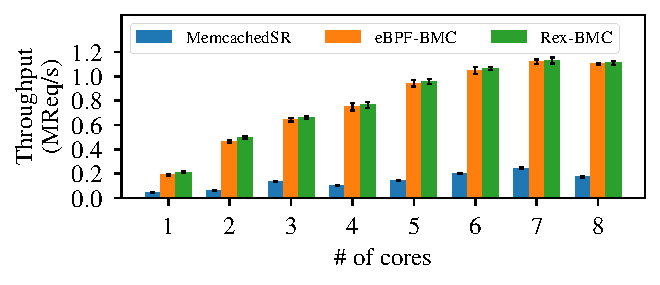
\includegraphics[width=1.0\linewidth]{figs/bmc.pdf}
    \centering
    \vspace{-25pt}
    \caption{Throughput of BMC on MemcachedSR, eBPF-BMC, and \projname{}-BMC
        under different number of CPUs/threads.
    }
    \label{fig:eval-bmc}
    \vspace{-10pt}
\end{figure}

Figure~\ref{fig:eval-bmc} shows the throughput of the three setups under
    different numbers of CPUs and threads.
MemcachedSR processes all requires in userspace and thus its throughput suffers
    from the overhead of the kernel network stack, achieving only 45K requests
    per second under a single thread and 175K requests per second under 8
    cores.
On the other hand, both eBPF-based and \projname{}-based BMC are able to
    achieve a much higher throughput because they can process a large
    fraction of requests at NIC level and without the need of going through
    the expensive kernel network stack.
With 8 CPU cores and threads, eBPF-BMC and \projname{}-BMC achieve a thoughput
    of 1.106M and 1.111M, and a performance benefit of 6.3x and 6.4x,
    respectively.
It is also clear that \projname{} is able achieve a better usability while
    keeping the same level of performance and safety guarrantee comparing to
    eBPF,  as the throughput of \projname{}-BMC is comparable to that of
    eBPF-BMC under all CPU/thread setups.
